%!TEX program = xelatex
\documentclass[a4paper,12pt]{report}
\usepackage{indentfirst} 
\usepackage{xeCJK}
\usepackage{times}
\usepackage{graphicx,float}
\usepackage{setspace}
\usepackage{fancyhdr}
\usepackage{array}
\usepackage{fontspec,xunicode,xltxtra}
\usepackage{titlesec}
\usepackage{titletoc}
\usepackage[titletoc]{appendix}
\usepackage[top=30mm,bottom=30mm,left=20mm,right=20mm]{geometry}
\usepackage{cite}
\usepackage{listings}
\usepackage[framed,numbered,autolinebreaks,useliterate]{mcode}
\usepackage[UTF8]{ctex}

\XeTeXlinebreaklocale "zh"
\XeTeXlinebreakskip = 0pt plus 1pt minus 0.1pt
\usepackage[linkbordercolor = white]{hyperref}

% 页眉页脚设置
\fancypagestyle{plain}{\pagestyle{fancy}}
\pagestyle{fancy}
\lhead{\kaishu 数据库实验报告}
\rhead{\kaishu 实验3}
\cfoot{\thepage}

% 章节标题设置
\titleformat{\chapter}{\centering\zihao{-1}\heiti}{实验\chinese{chapter}}{1em}{}
\titlespacing{\chapter}{0pt}{*0}{*6}

% 代码样式配置
\setCJKfamilyfont{simsun}{SimSun}
\setCJKfamilyfont{SimHei}{SimHei}
\lstset{
    language=SQL,
    basicstyle=\ttfamily\small\CJKfamily{simsun},
    commentstyle=\color{green!50!black},
    keywordstyle=\color{blue},
    stringstyle=\color{red},
    showstringspaces=false,
    breaklines=true,
    frame=single,
    numbers=left,
    numberstyle=\tiny\color{gray},
    escapeinside=``,
    literate={。}{{。}}1
            {，}{{，}}1
            {'}{{\textquotesingle}}1 % 处理单引号
            {`}{{\textbacktick}}1 % 处理反引号
            {_}{{\textunderscore}}1 % 处理下划线
}

\setCJKfamilyfont{kai}{KaiTi}
\setlength{\headheight}{14.49998pt}

% 定义封面宏
\newcommand{\makeExperimentCover}[7]{
    \begin{titlepage}
        \begin{center}
            
\includegraphics[width=1.0\textwidth]{figure/nankai.jpg}\\
            \vspace{50mm}
            \textbf{\zihao{1}\heiti{#1}}\\[1cm]
            \textbf{\zihao{2}\heiti{(2024\textasciitilde2025学年第二学期)}}\\[1cm]
            \vspace{\fill}
            
            \setlength{\extrarowheight}{2mm}
            {\songti\zihao{3}	
            \begin{tabular}{rl}
                 实验名称：& MySQL数据库综合操作实验\\
                 学\qquad 院：& 软件学院\\
                 姓\qquad 名：& 郭威威\\
                 学\qquad 号：& 2414308\\
                 指导老师：& 李旭东\\
            \end{tabular}
            }\\[2cm]
            \vspace{\fill}
            \zihao{4}
            2024\textasciitilde 2025春季学期\\
            使用\LaTeX 撰写于 \today
        \end{center}	
    \end{titlepage}
}

\begin{document}
% 调用封面宏生成封面
\makeExperimentCover{MySQL数据库综合操作实验}{MySQL数据库综合操作实验}{软件学院}{郭威威}{2414308}{李旭东}

% 目录
\tableofcontents

% 正文内容区域
\begin{spacing}{1.5}
\songti\zihao{-4}

\chapter{实验目的}
掌握Python与MySQL数据库的交互方法，熟练进行数据库表结构设计、数据操作及复杂查询，理解外键约束的应用与数据完整性管理，提升数据库综合操作能力。

\chapter{实验环境}
\section{操作系统}
Windows 11 Pro 22H2

\section{软件版本}
\begin{table}[H]
    \centering
    \begin{tabular}{|l|l|}
        \hline
        软件名称 & 版本号 \\
        \hline
        MySQL & 8.0.41 \\
        MySQL Workbench & 8.0.36 \\
        Python & 3.11 \\
        PyMySQL & 1.1.1 \\
        \hline
    \end{tabular}
    \caption{实验软件版本信息}
\end{table}

\chapter{实验步骤}
\section{Python数据库连接}
\subsection{初始连接问题}
首次使用错误数据库导致异常：
\begin{lstlisting}[language=bash]
pymysql.err.ProgrammingError: (1146, "Table 'sys.teacher' doesn't exist")
\end{lstlisting}
\begin{center}
    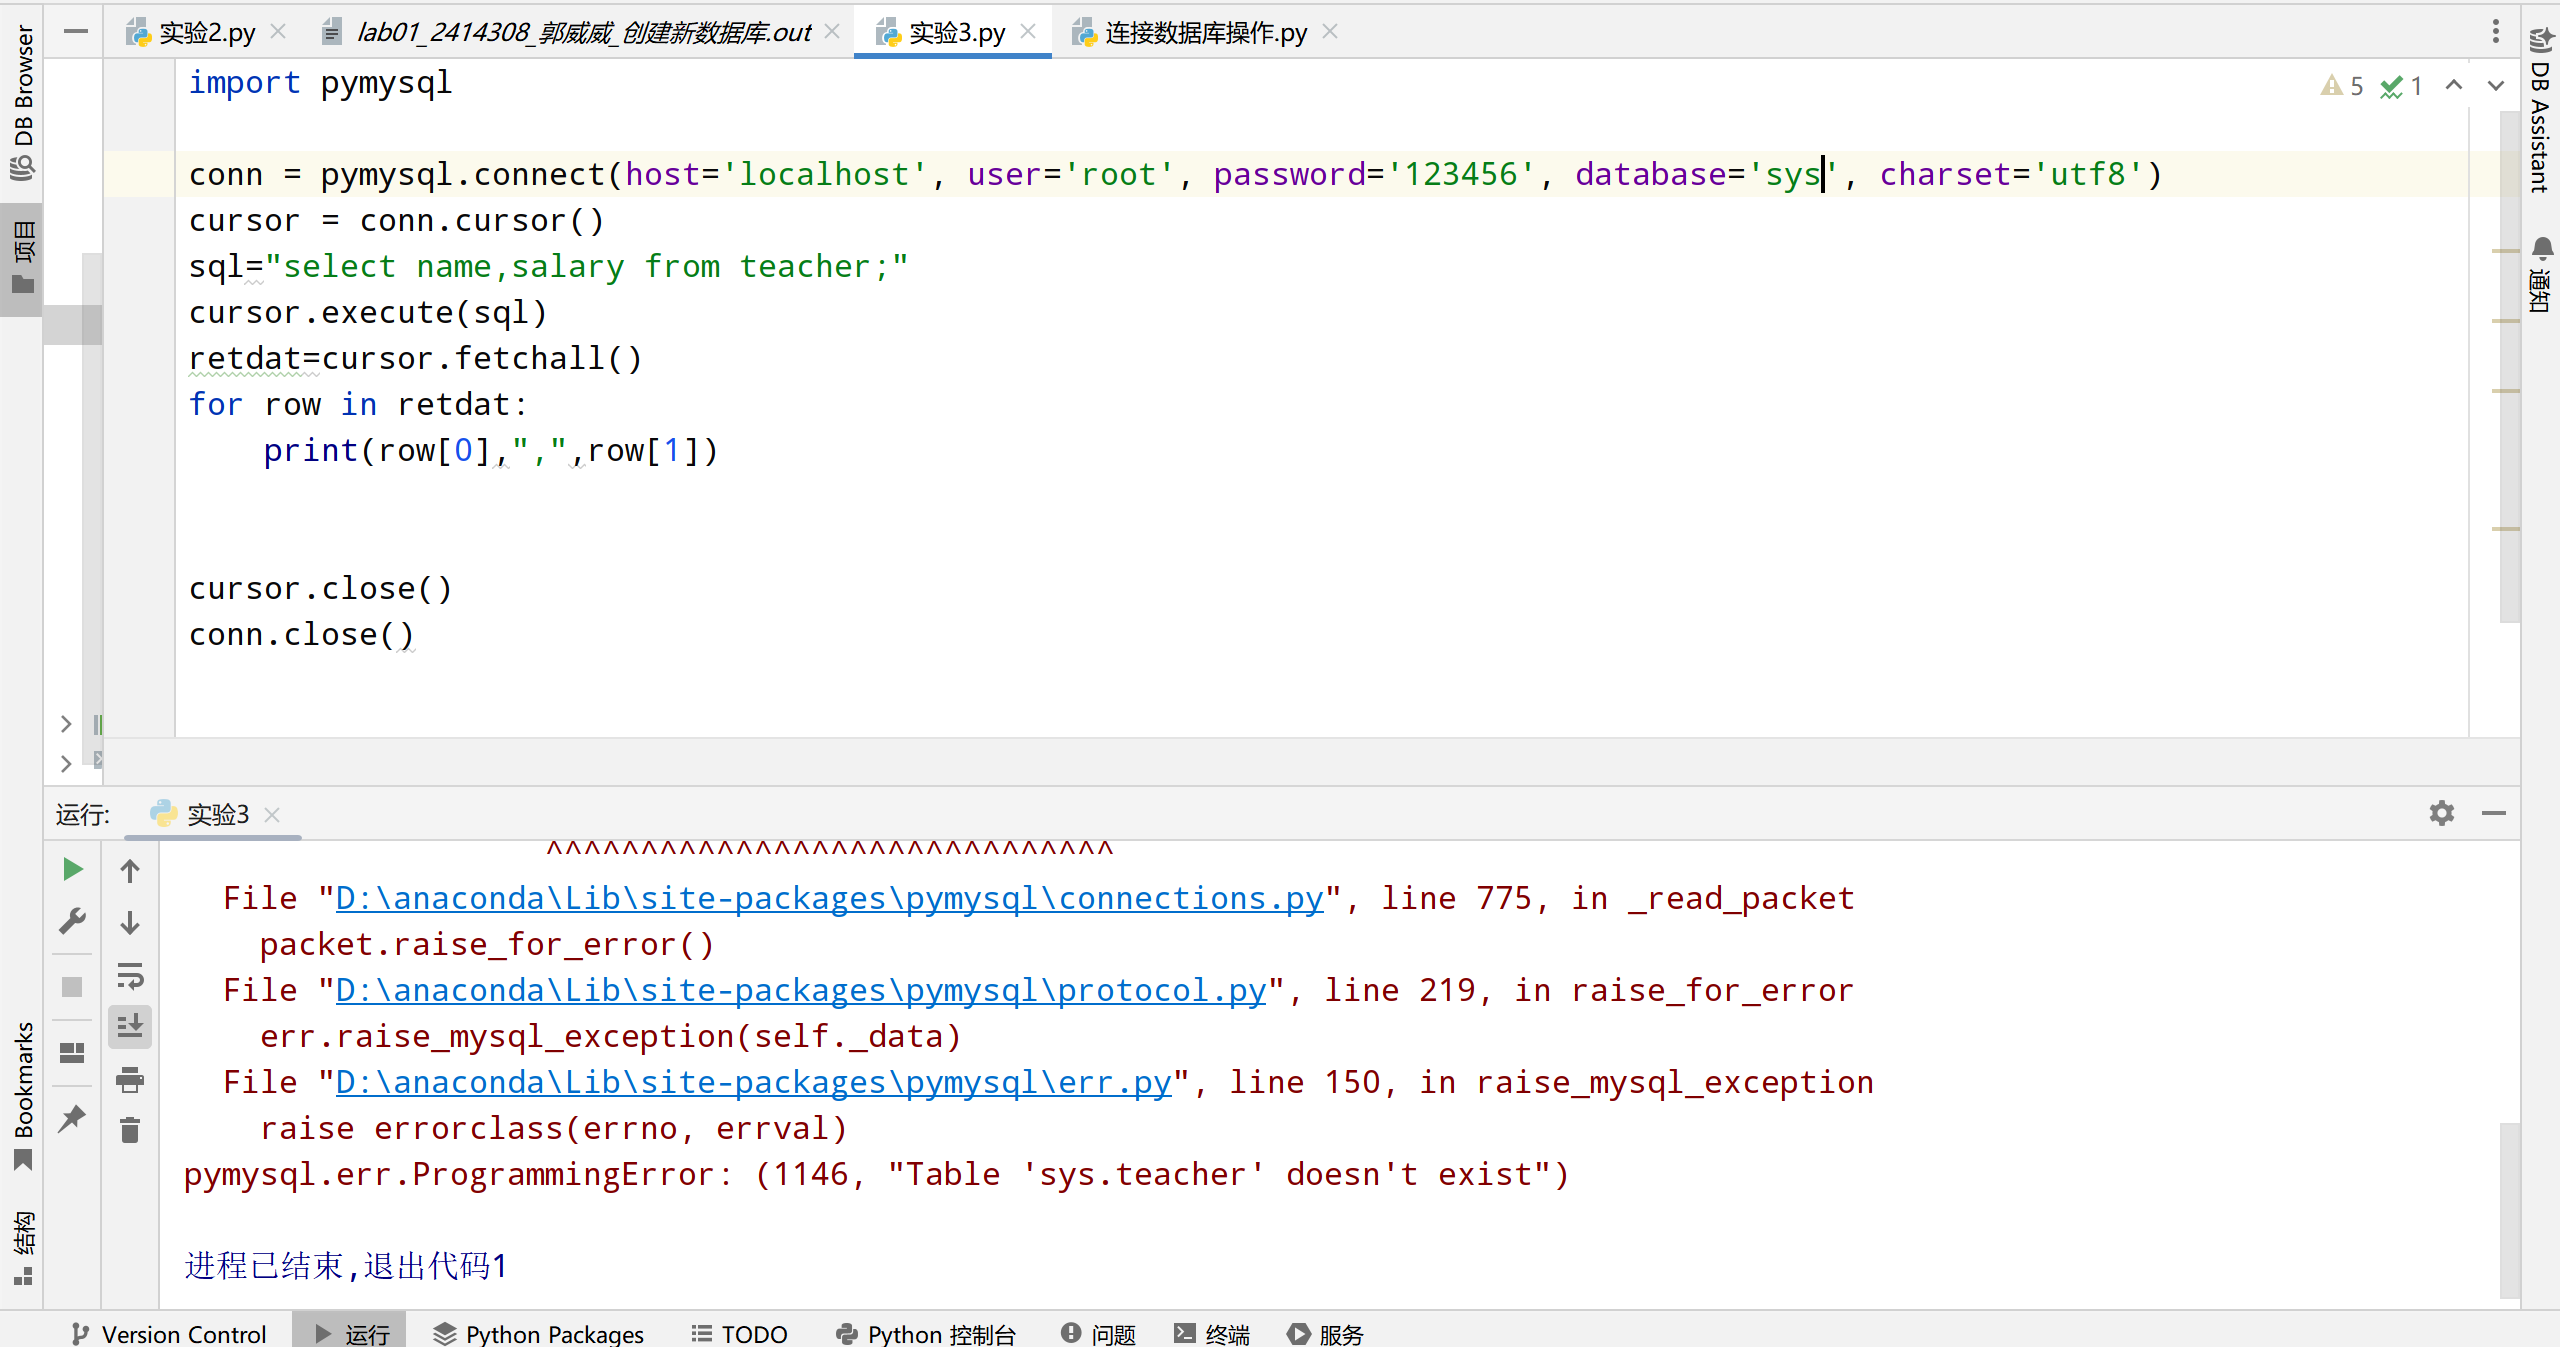
\includegraphics[width=12cm]{figure/image1.png} \\
    \footnotesize 图1 Python数据库连接错误截图
\end{center}
\vspace{1cm}

修改数据库连接参数后仍因用户名错误导致：
\begin{lstlisting}[language=bash]
pymysql.err.OperationalError: (1045, "Access denied for user 'myuserco'@'localhost'")
\end{lstlisting}
\begin{center}
    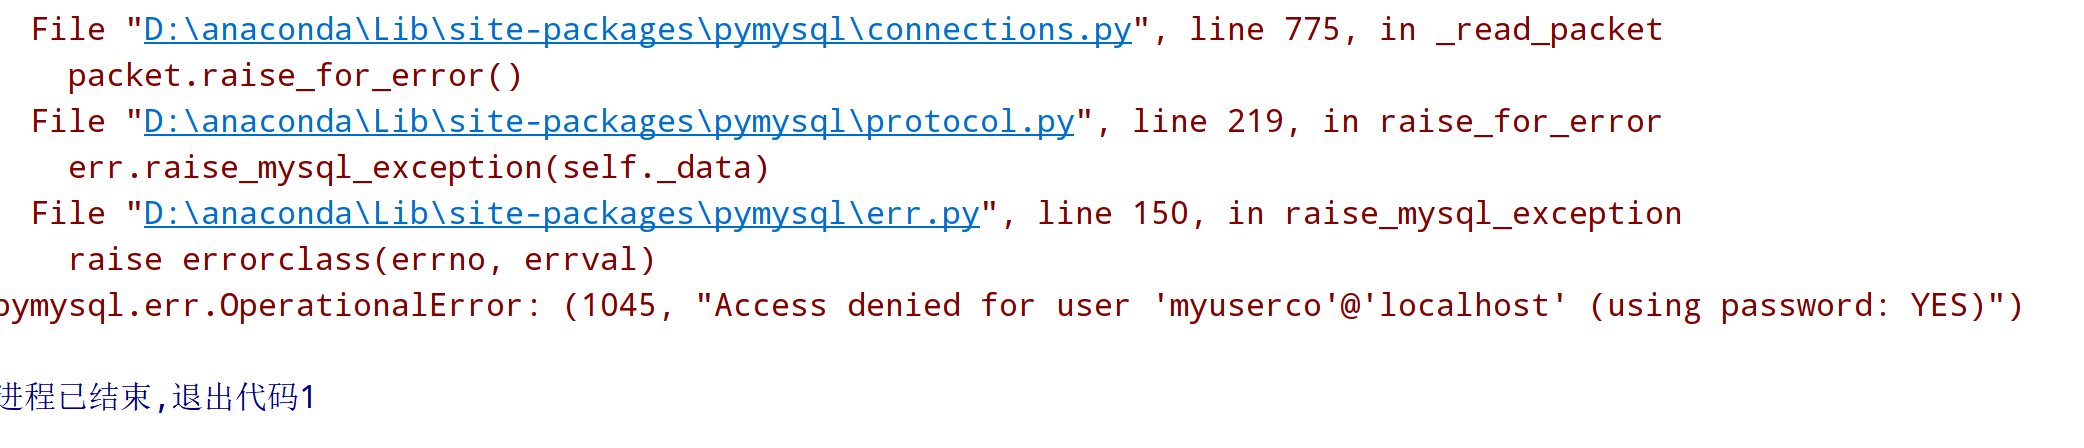
\includegraphics[width=12cm]{figure/image2.png} \\
    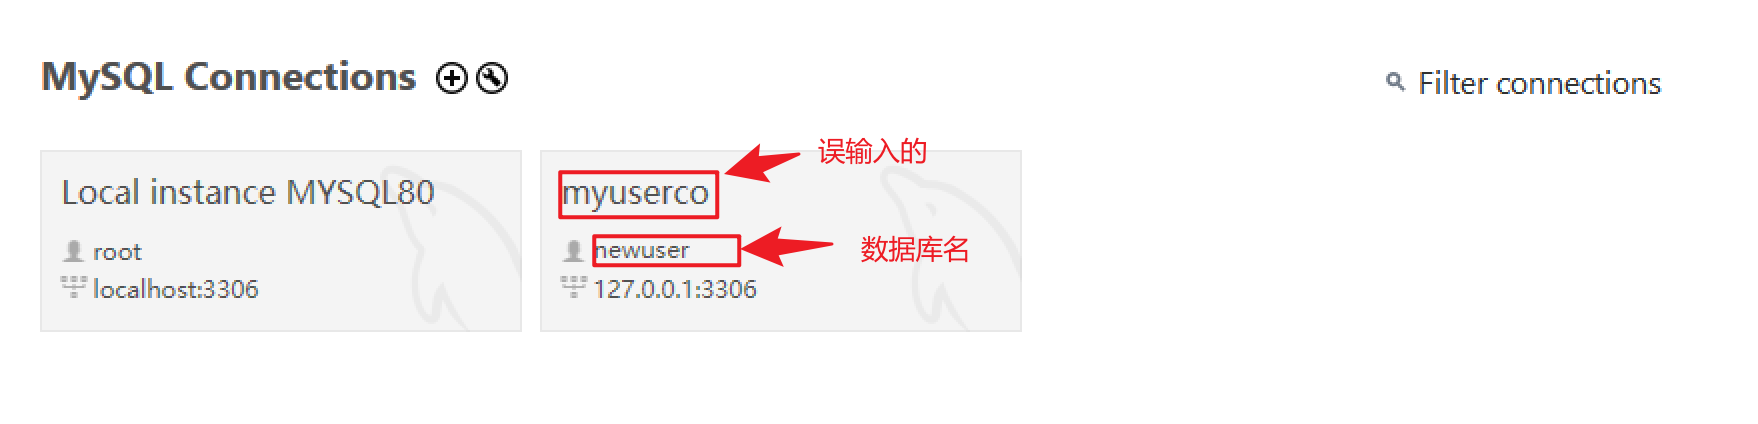
\includegraphics[width=12cm]{figure/image3.png} \\
    \footnotesize 图2、3 MySQL连接配置错误截图
\end{center}
\vspace{1cm}

再次运行后发现原数据库中没有teacher表：
\begin{lstlisting}[language=bash]
pymysql.err.ProgrammingError: (1146, "Table 'dbsclab2025.teacher' doesn't exist")
\end{lstlisting}
\begin{center}
    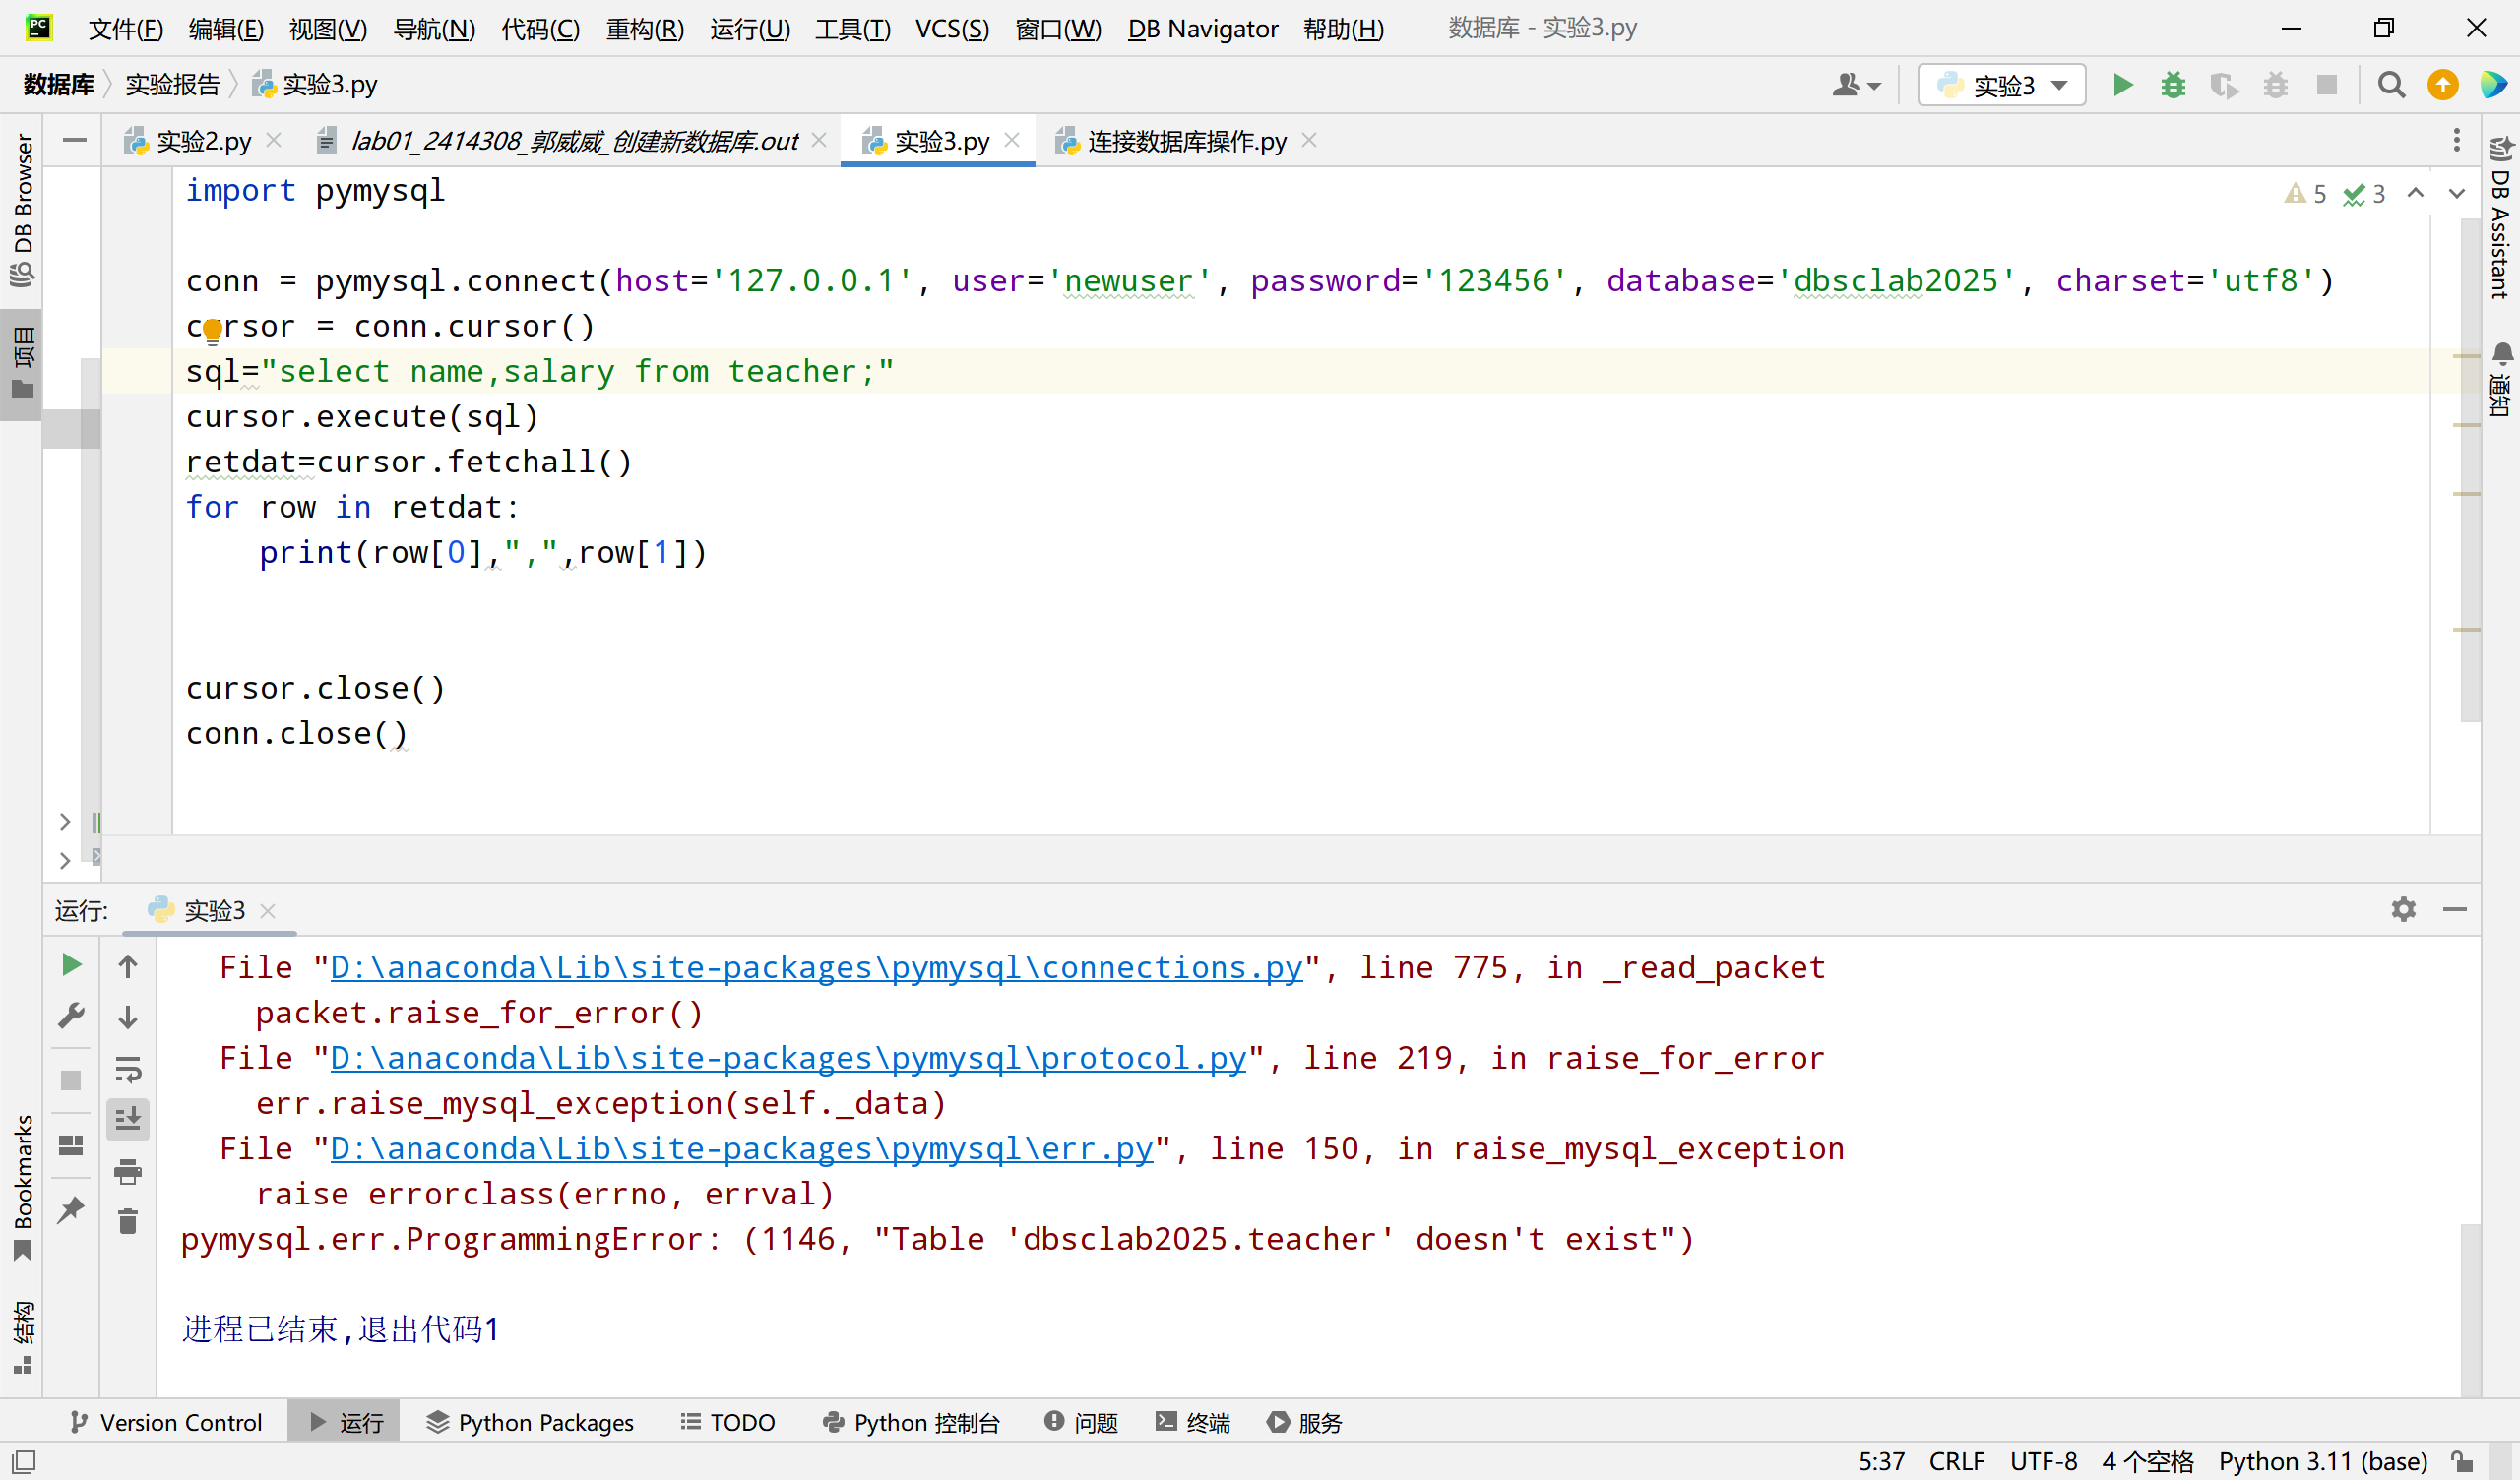
\includegraphics[width=12cm]{figure/image4.png} \\
    \footnotesize 图4 数据库表不存在错误截图
\end{center}
\vspace{1cm}

\subsection{正确连接配置}
最终使用正确参数连接成功：改成instructor表后成功显示数据
\begin{lstlisting}[language=Python]
import pymysql
conn = pymysql.connect(
    host='127.0.0.1',
    user='newuser',
    password='123456',
    database='dbsclab2025',
    charset='utf8'
)
cursor = conn.cursor()
cursor.execute("SELECT name, salary FROM instructor")
for row in cursor.fetchall():
    print(f"{row[0]}, {row[1]}")
cursor.close()
conn.close()
\end{lstlisting}
运行结果显示：
\begin{lstlisting}[language=bash]
Lembr, 32241.56
Bawa, 72140.88
Yazdi, 98333.65
Wieland, 124651.41
DAgostino, 59706.49
Liley, 90891.69
Kean, 35023.18
Atanassov, 84982.92
Moreira, 71351.42
\end{lstlisting}
\begin{center}
     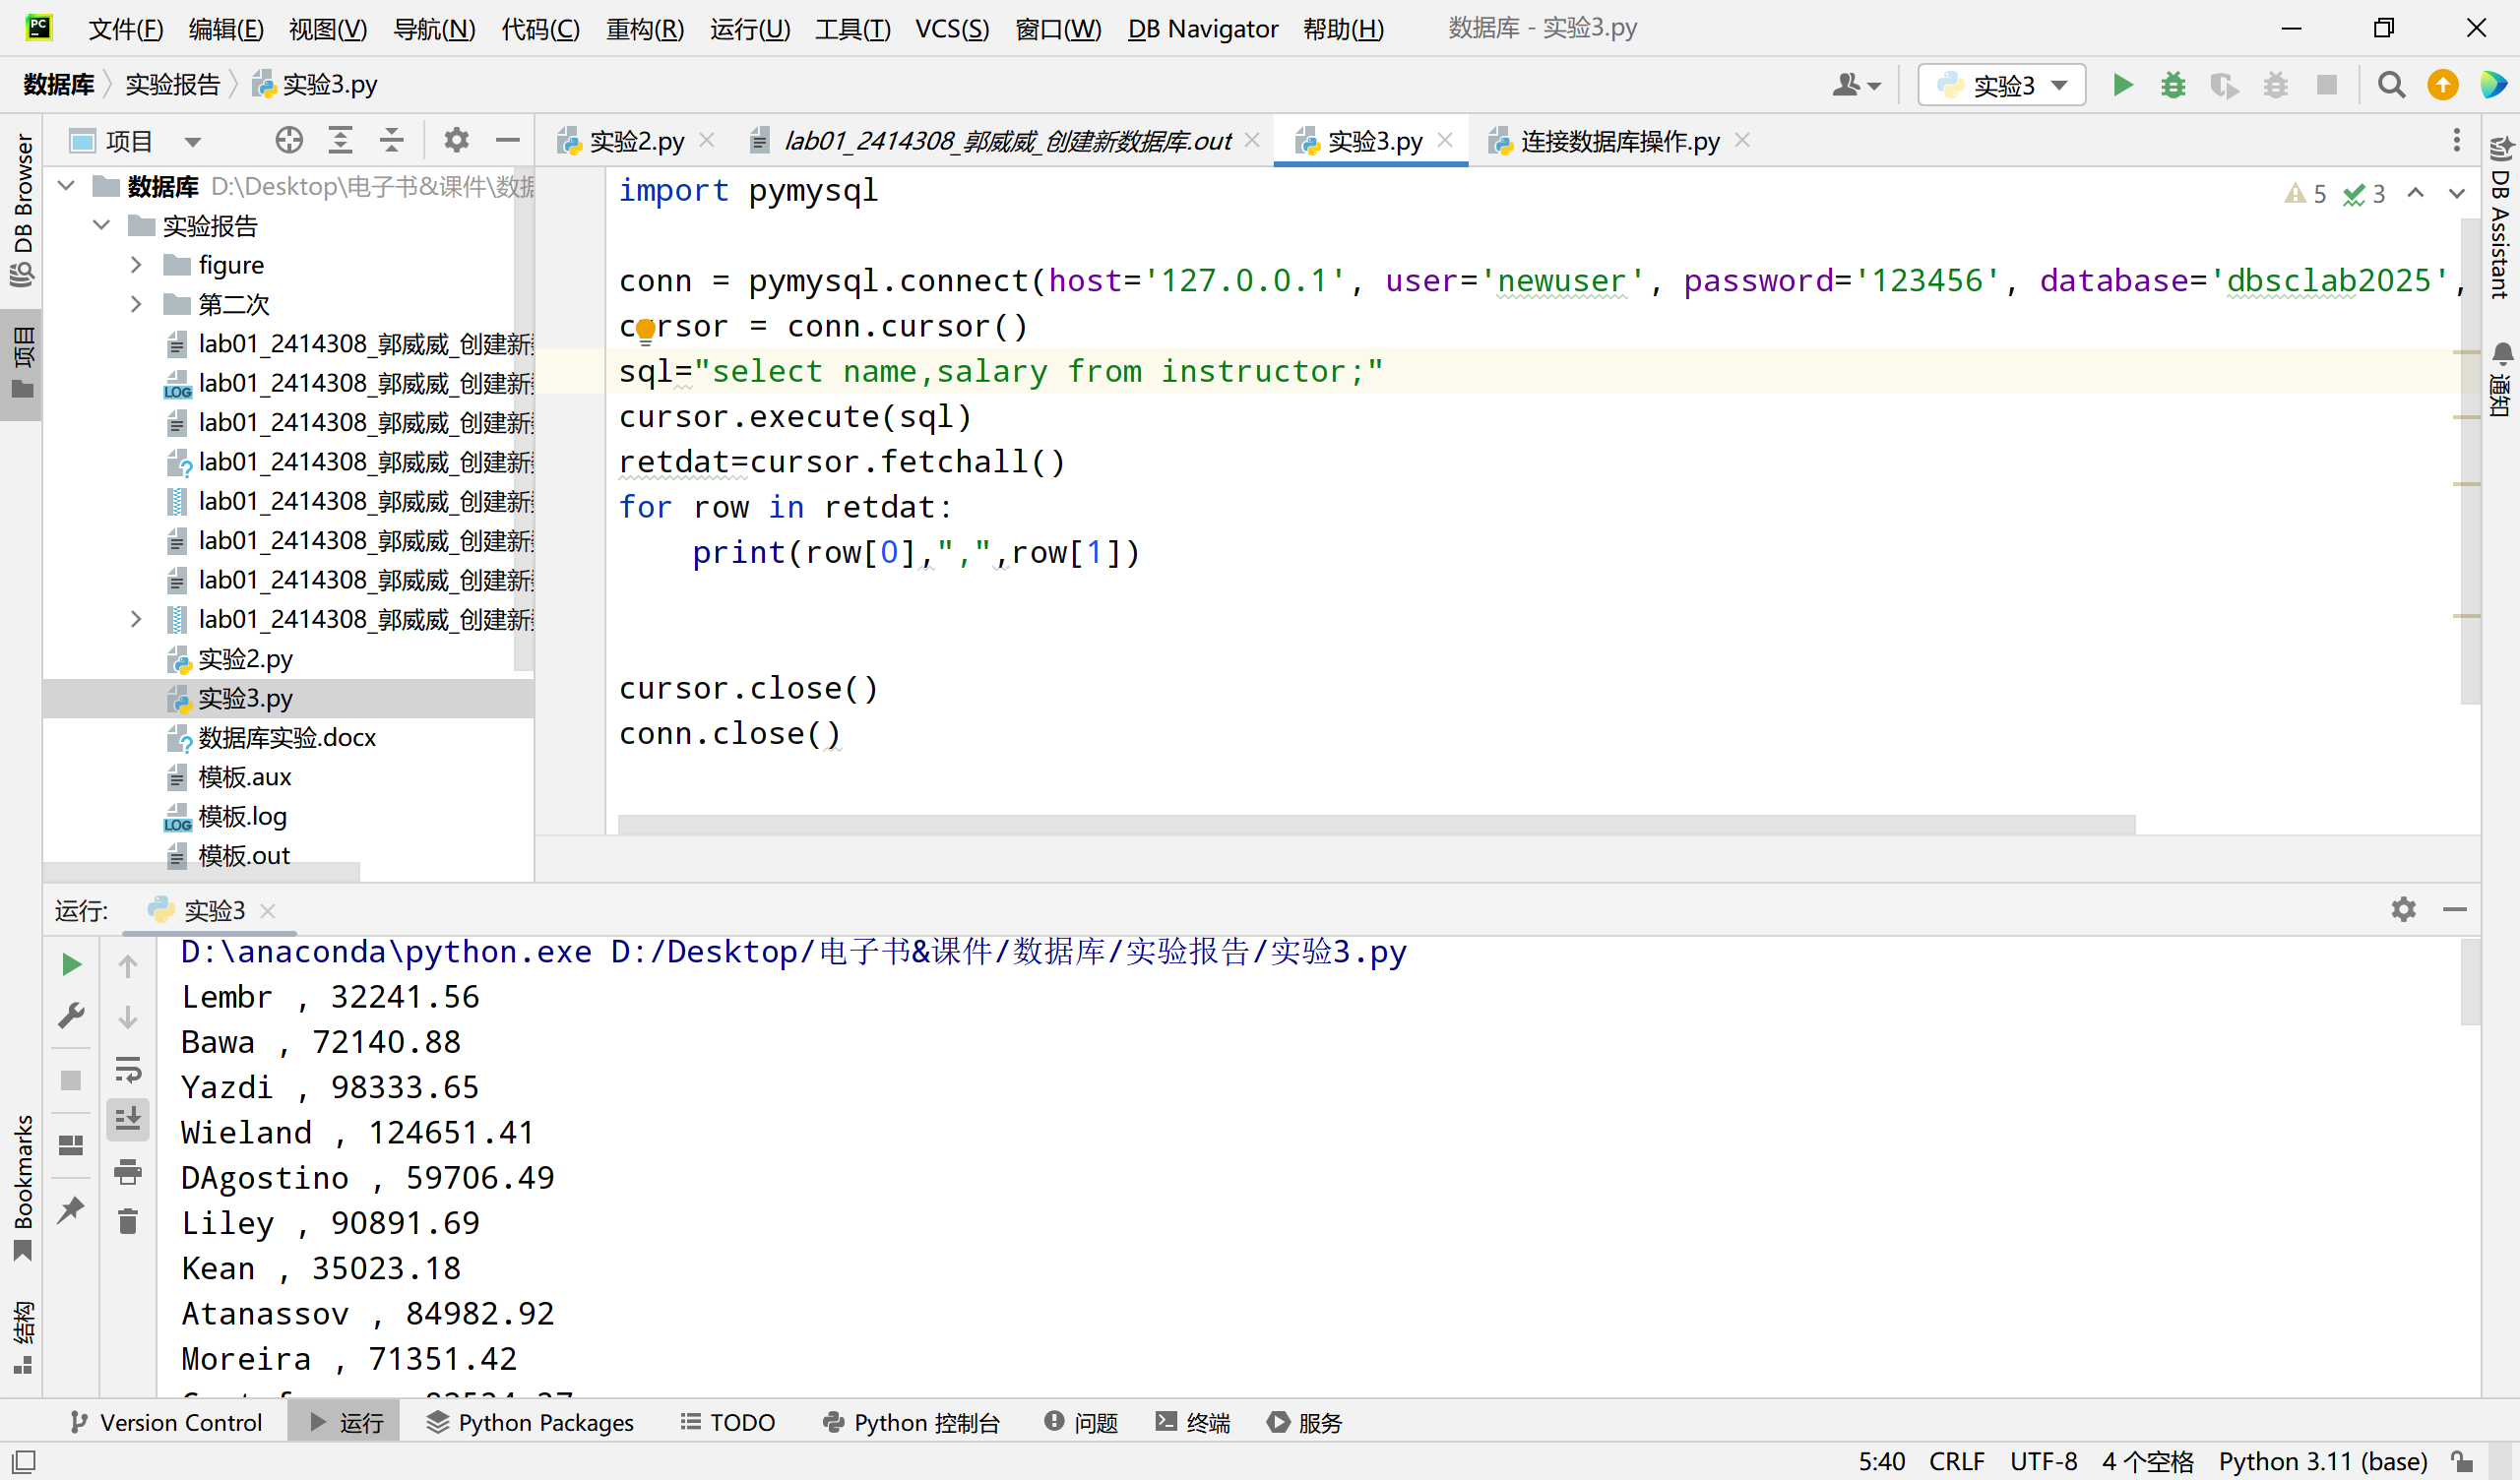
\includegraphics[width=12cm]{figure/image5.png} \\
    \footnotesize 图5 Python连接成功结果截图
\end{center}
\vspace{1cm}

\section{数据库表设计（DDL）}
\subsection{创建基础表}
\begin{lstlisting}[language=SQL]
CREATE TABLE department01 (
    deptname VARCHAR(255) PRIMARY KEY,
    location VARCHAR(255)
);

CREATE TABLE student01 (
    ID INT PRIMARY KEY,
    Name VARCHAR(255),
    Birthplace VARCHAR(255)
);
\end{lstlisting}
\begin{center}
    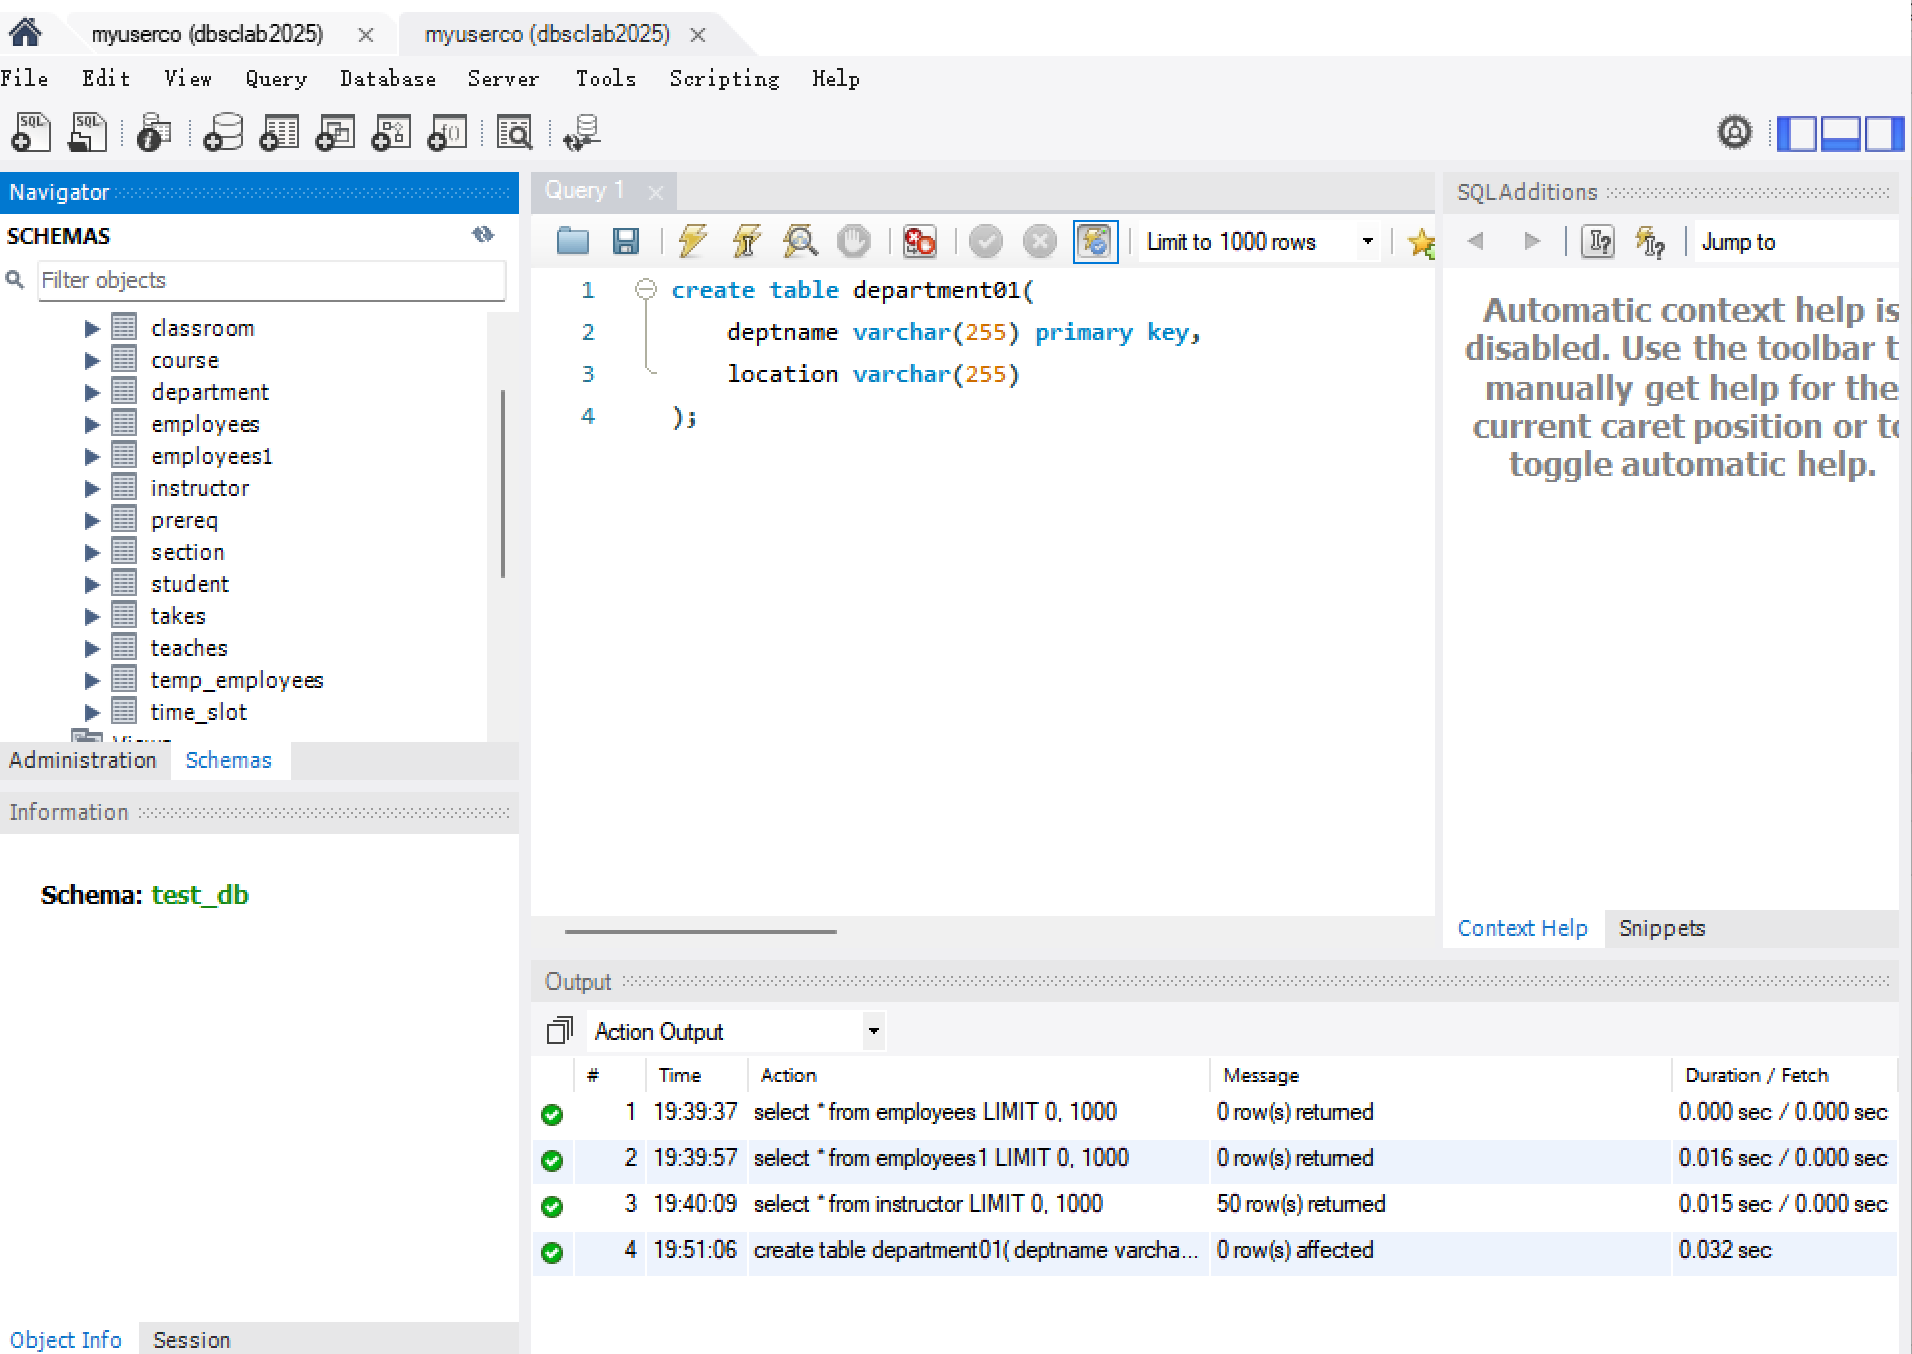
\includegraphics[width=12cm]{figure/image6.png} \\
    \footnotesize 图6 创建department01表操作截图
\end{center}
\vspace{1cm}
\begin{center}
    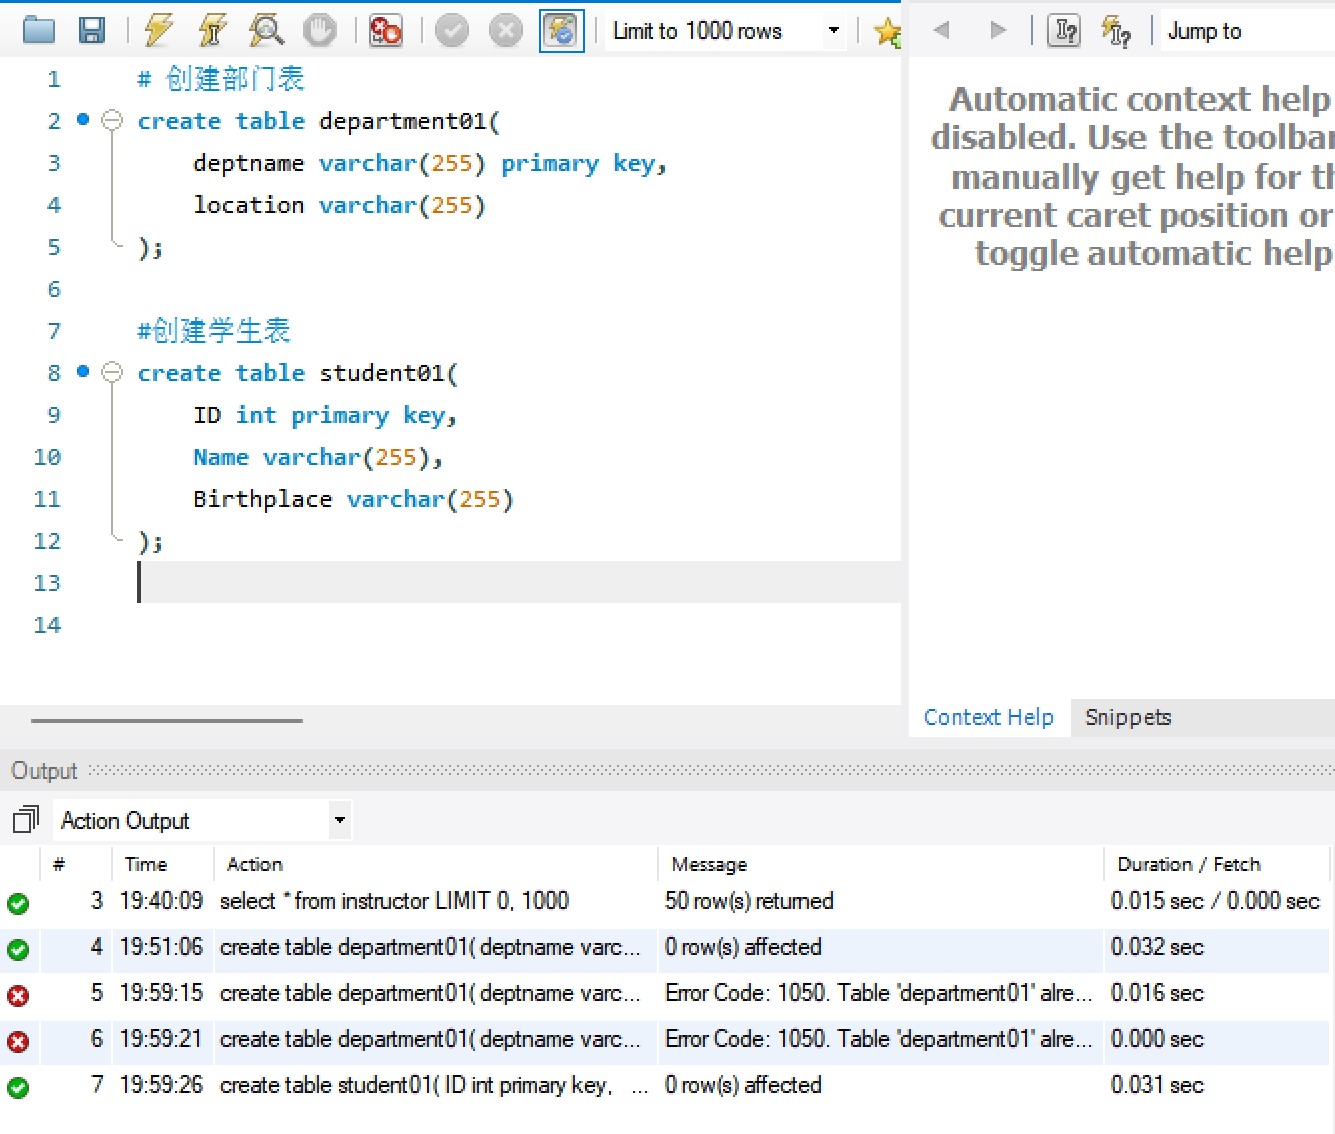
\includegraphics[width=12cm]{figure/image7.png} \\
    \footnotesize 图7 创建student01表操作截图
\end{center}
\vspace{1cm}

\subsection{添加外键约束}
增加外键时出错，单行运行后成功运行
\begin{lstlisting}[language=SQL]
ALTER TABLE student01 
ADD COLUMN deptname VARCHAR(255),
ADD FOREIGN KEY (deptname) REFERENCES department01(deptname);
\end{lstlisting}
\begin{center}
    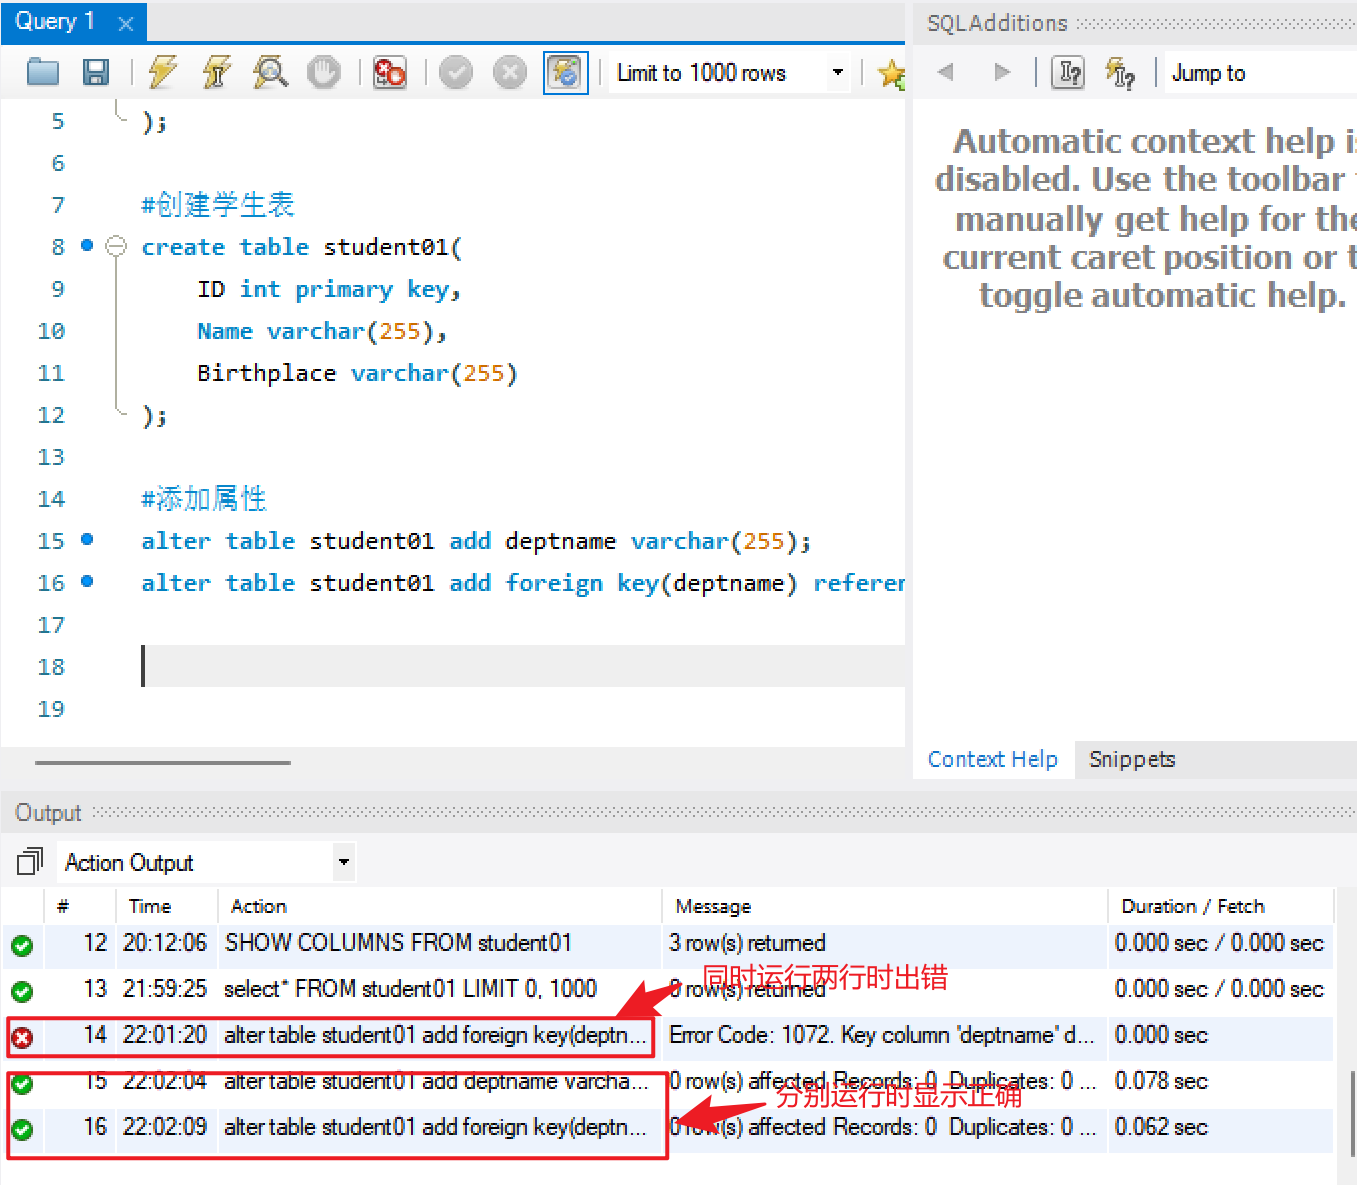
\includegraphics[width=12cm]{figure/image8.png} \\
    \footnotesize 图8 添加外键约束截图
\end{center}
\vspace{1cm}

\subsection{数据完整性管理}
通过外键约束实现数据依赖，插入数据时需保证外键存在：向student01插入数据出错，发现外键不对应引起增加相应外键
\begin{lstlisting}[language=SQL]
INSERT INTO department01(deptname) VALUES ('cs'), ('ee'), ('me'), ('ce');
INSERT INTO student01 (ID, Name, Birthplace, deptname) VALUES
(1, 'alice', 'new york', 'cs'),
(2, 'bob', 'chicago', 'ee'),
(3, 'charlie', 'los angeles', 'me'),
(4, 'david', 'houston', 'ce'),
(5, 'eve', 'phoenix', 'cs');
\end{lstlisting}
\begin{center}
    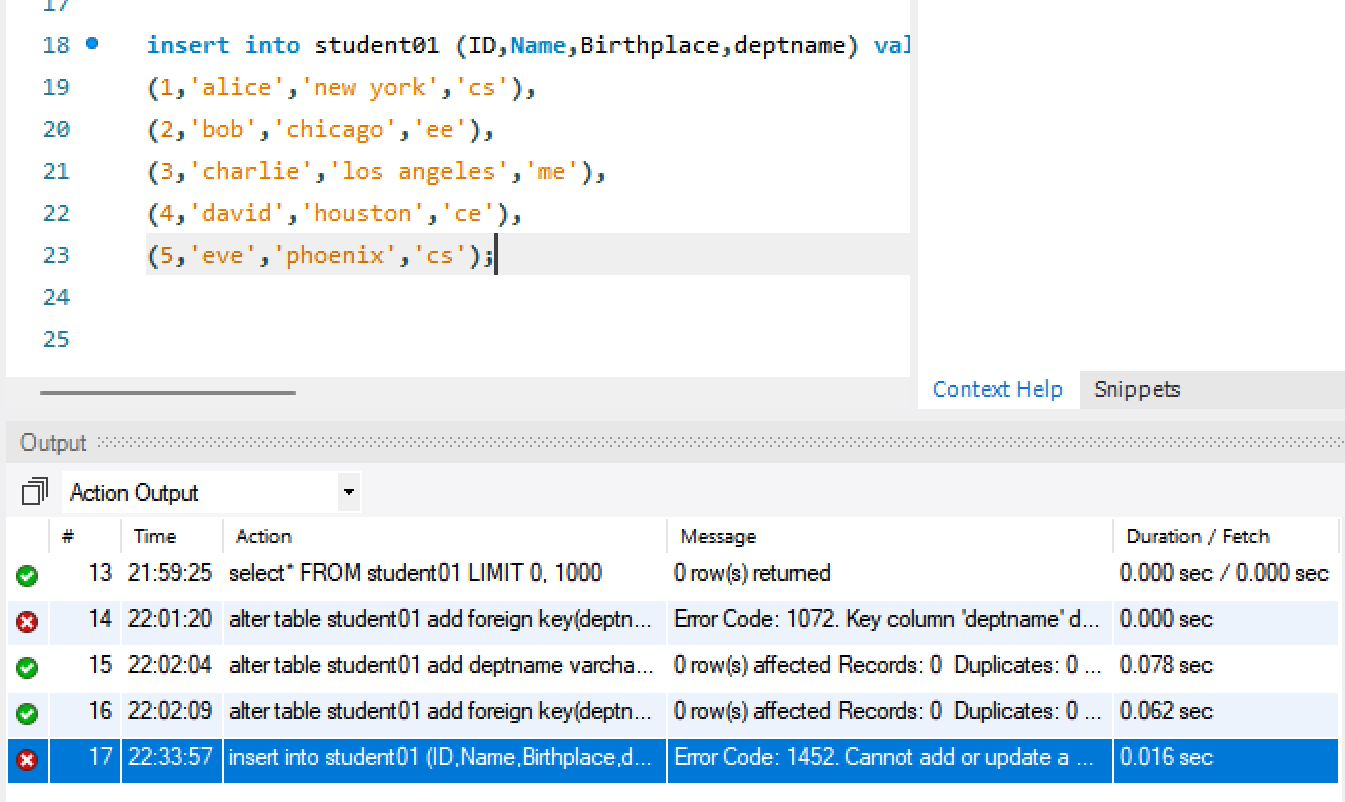
\includegraphics[width=12cm]{figure/image9.png} \\
    \footnotesize 图9 部门表数据插入截图
\end{center}
\vspace{1cm}
增加相应外键后成功：
\begin{center}
    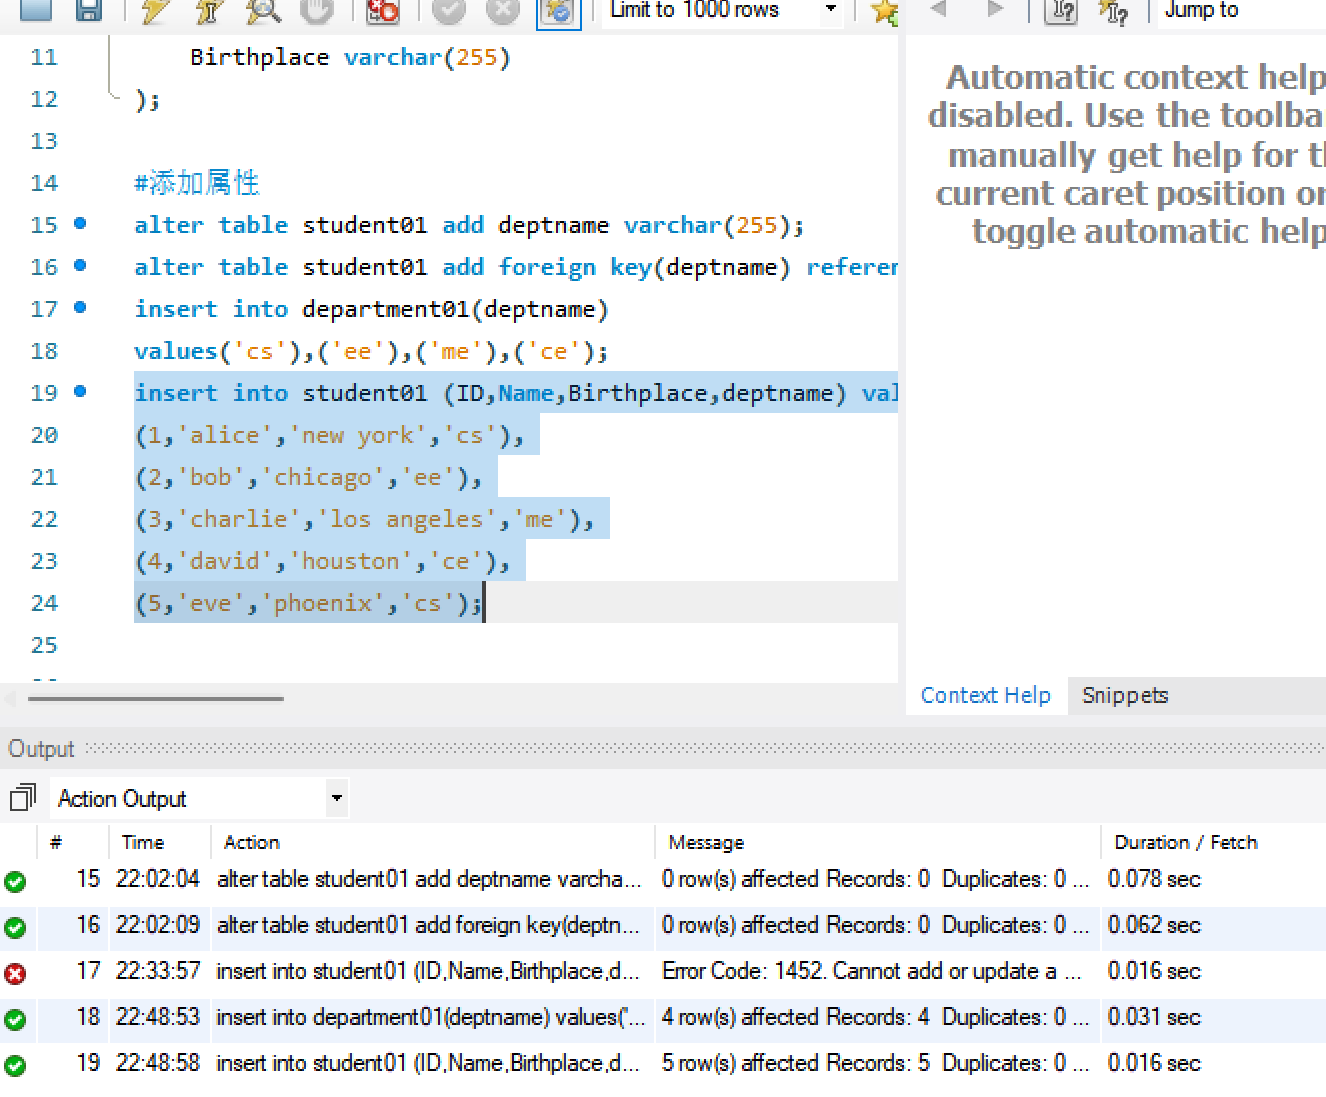
\includegraphics[width=12cm]{figure/image10.png} \\
    \footnotesize 图10 学生表数据插入截图
\end{center}
\vspace{1cm}
\subsection{删除}
删除表失败，发现student01引用了department01的外键
\begin{center}
    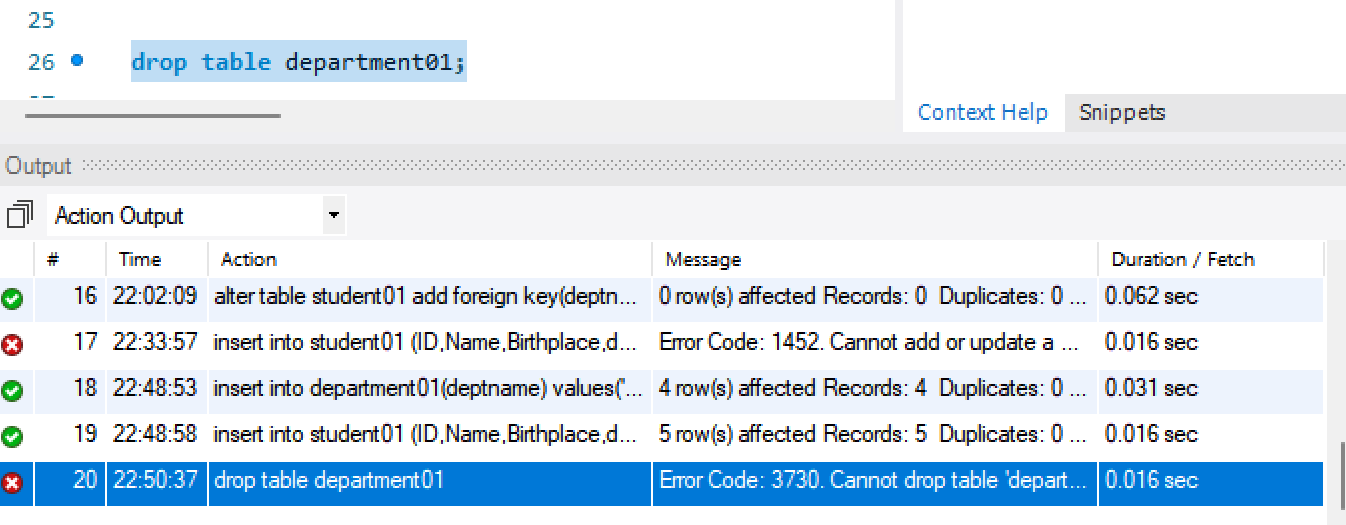
\includegraphics[width=12cm]{figure/image11.png} \\
    \footnotesize 图11 数据删除操作截图1
\end{center}
\vspace{1cm}
将student01表中对department01表的外键引用删除，删除后成功
\begin{center}
    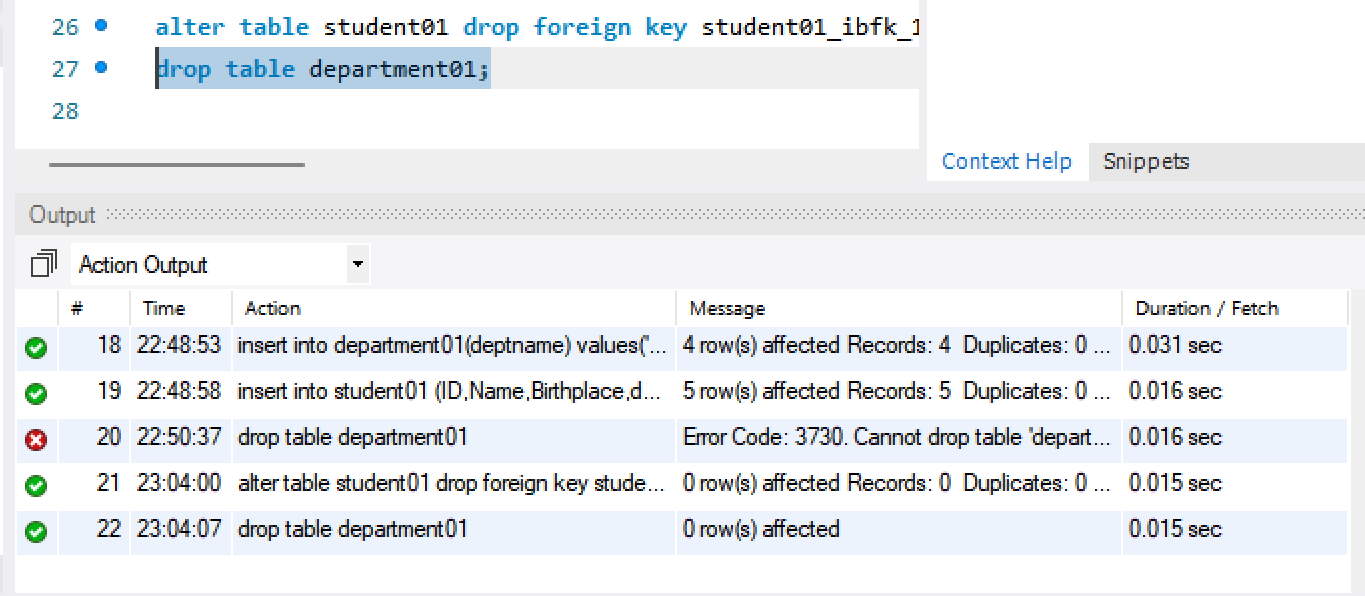
\includegraphics[width=12cm]{figure/image12.png} \\
    \footnotesize 图12 数据删除操作截图2
\end{center}
\vspace{1cm}

\section{数据操作（DML）}
\subsection{数据导入}
注意导入的数据之间一一对应
\begin{lstlisting}[language=SQL]
INSERT INTO student01(ID, Name, Birthplace, deptname) 
SELECT ID, name, NULL, dept_name FROM student;
\end{lstlisting}
\begin{center}
    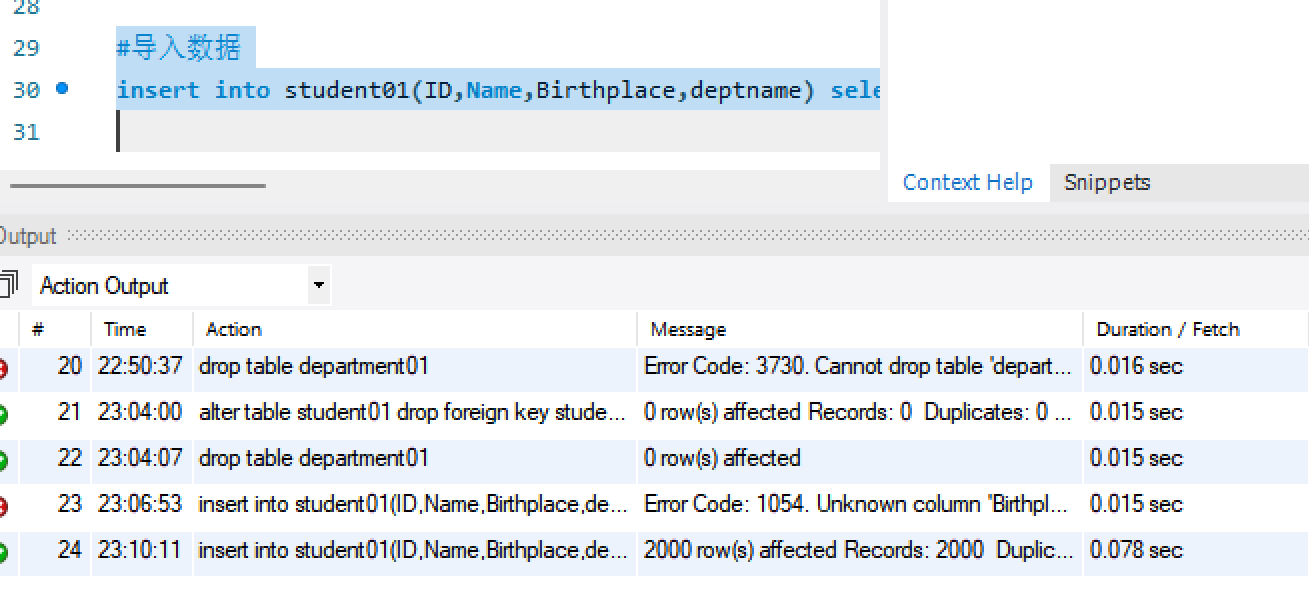
\includegraphics[width=12cm]{figure/image13.png} \\
    \footnotesize 图13 数据导入操作截图
\end{center}
\vspace{1cm}

\subsection{数据检索}
\begin{lstlisting}[language=SQL]
SELECT Name, deptname FROM student01;
\end{lstlisting}
\begin{center}
    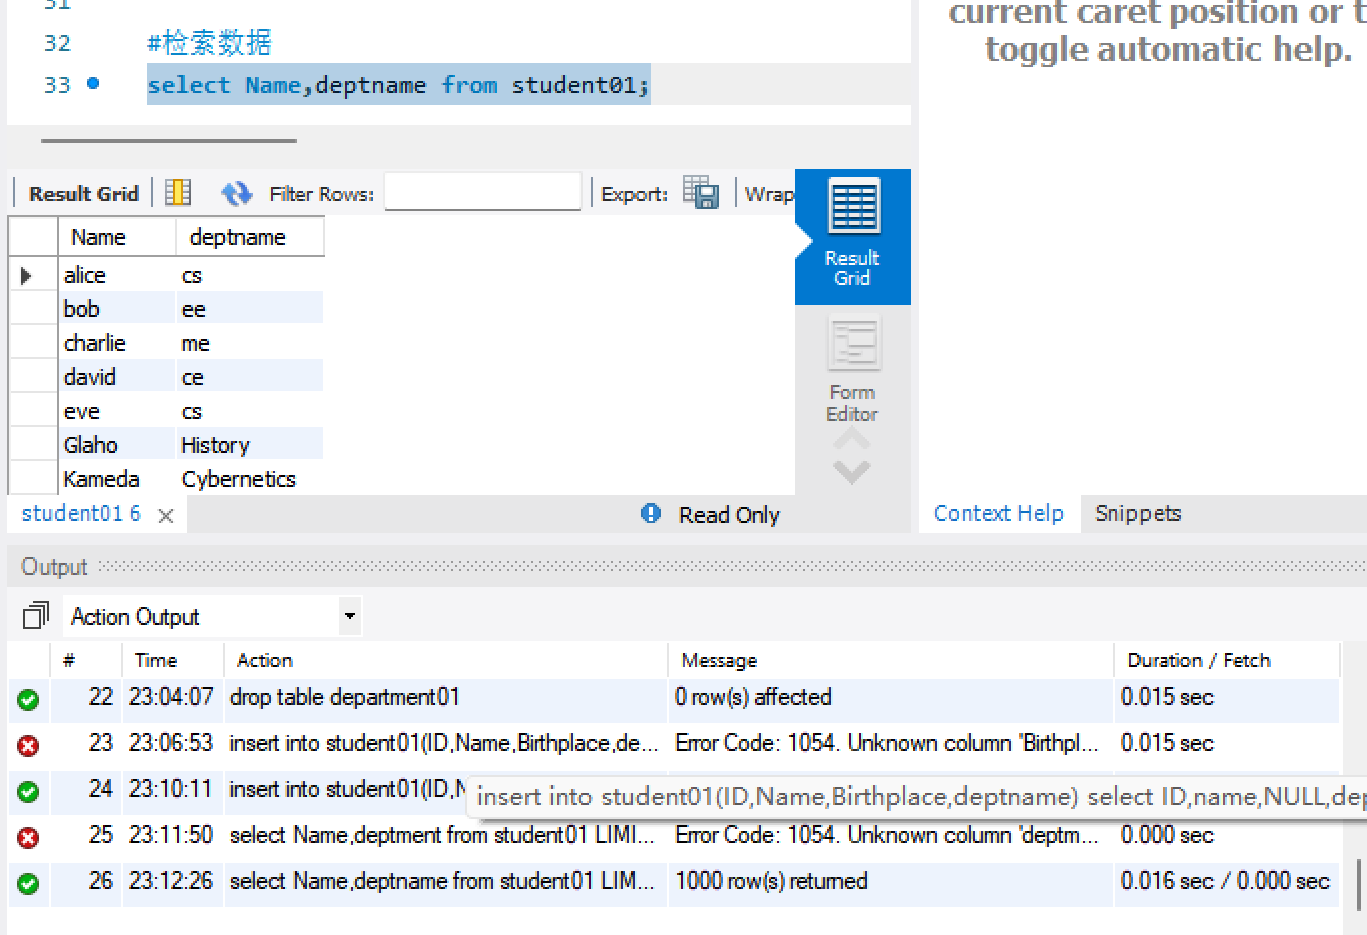
\includegraphics[width=12cm]{figure/image14.png} \\
    \footnotesize 图14 数据检索操作截图
\end{center}
\vspace{1cm}

\subsection{数据更新}
\begin{lstlisting}[language=SQL]
UPDATE student01 SET Birthplace='Unknown';
\end{lstlisting}
\begin{center}
    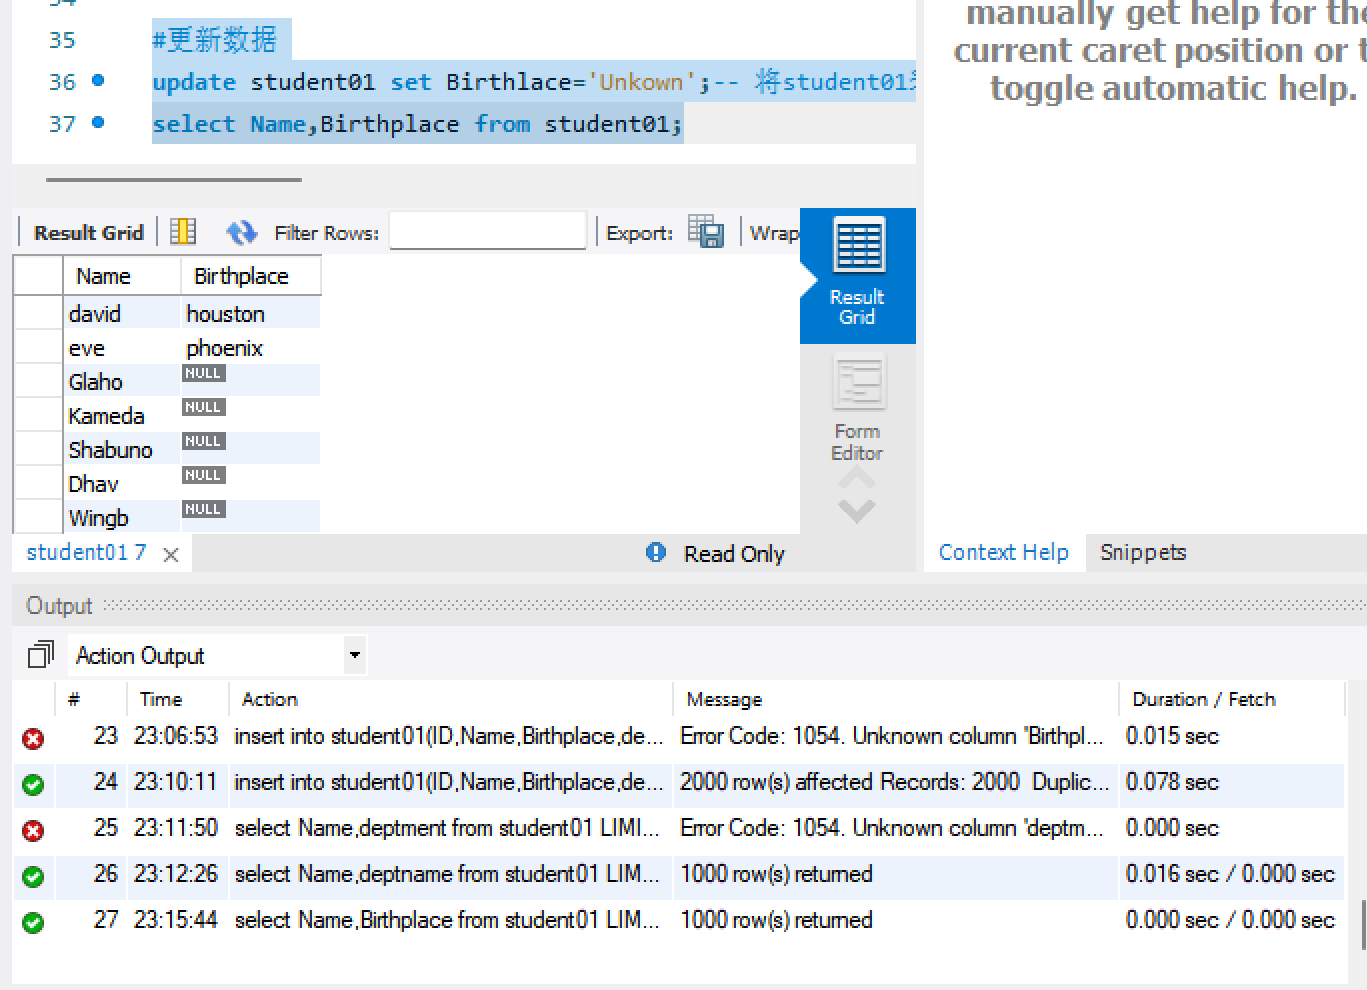
\includegraphics[width=12cm]{figure/image15.png} \\
    \footnotesize 图15 数据更新操作截图
\end{center}
\vspace{1cm}

\subsection{数据删除}
\begin{lstlisting}[language=SQL]
DELETE FROM student01 WHERE deptname="Comp.Sci.";
\end{lstlisting}
\begin{center}
    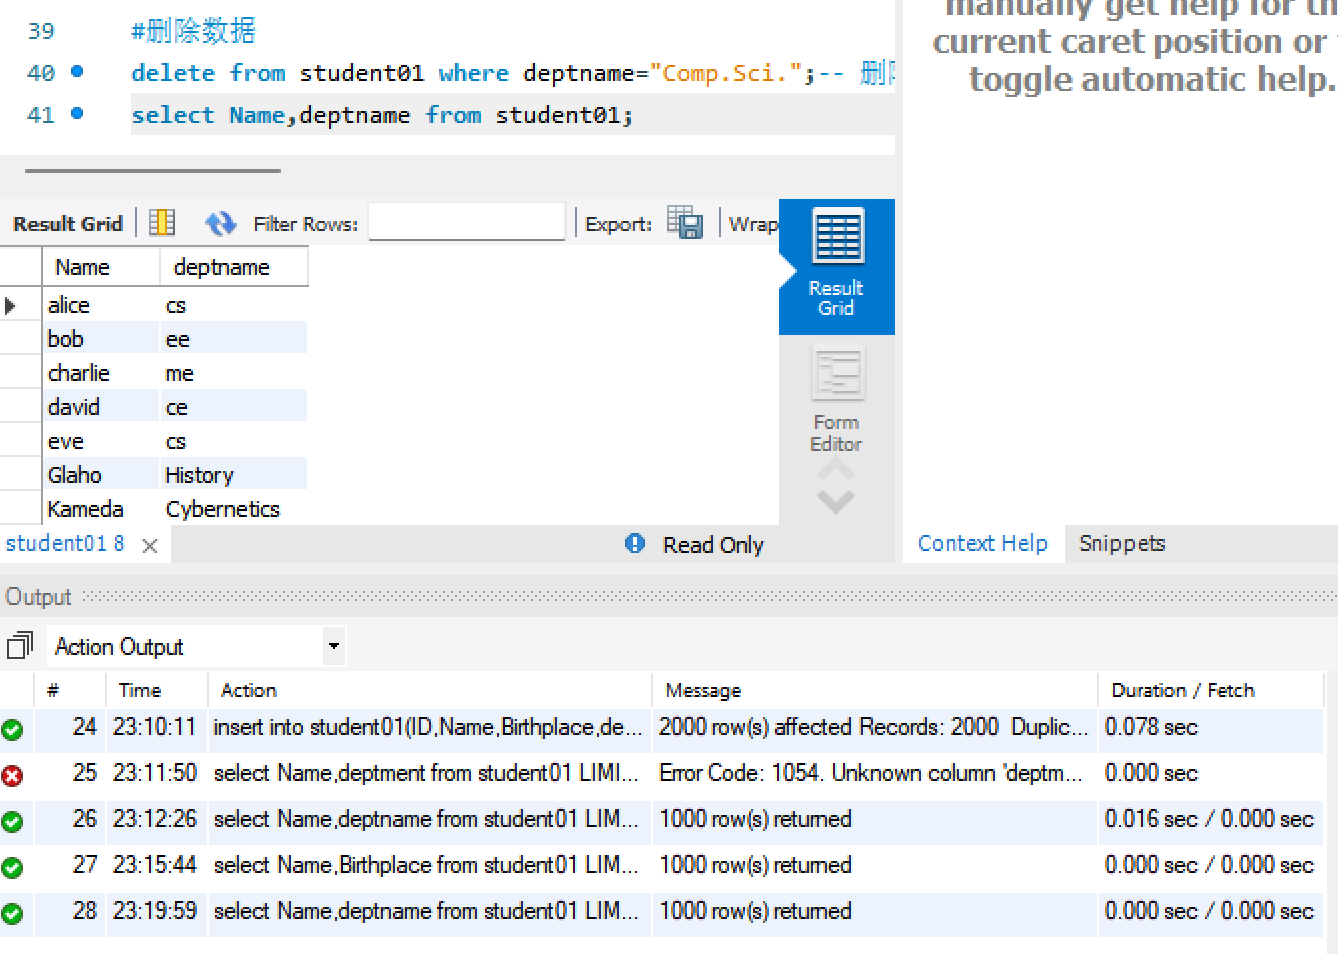
\includegraphics[width=12cm]{figure/image16.png} \\
    \footnotesize 图16 数据删除操作截图
\end{center}
\vspace{1cm}

\chapter{实验结果}
\section{数据库操作验证}
\subsection{表结构验证}
\begin{lstlisting}[language=SQL]
SHOW CREATE TABLE student01;
\end{lstlisting}
输出显示表结构包含外键约束：
\begin{lstlisting}[language=SQL]
CREATE TABLE `student01` (
  `ID` int NOT NULL,
  `Name` varchar(255) DEFAULT NULL,
  `Birthplace` varchar(255) DEFAULT NULL,
  `deptname` varchar(255) DEFAULT NULL,
  PRIMARY KEY (`ID`),
  KEY `student01\_ibfk\_1` (`deptname`),
  CONSTRAINT `student01\_ibfk\_1` FOREIGN KEY (`deptname`) REFERENCES `department01` (`deptname`)
) ENGINE=InnoDB DEFAULT CHARSET=utf8mb4
\end{lstlisting}

\subsection{数据完整性验证}
删除部门表前需先删除外键约束：
\begin{lstlisting}[language=SQL]
ALTER TABLE student01 DROP FOREIGN KEY student01_ibfk_1;
DROP TABLE department01;
\end{lstlisting}
\begin{center}
    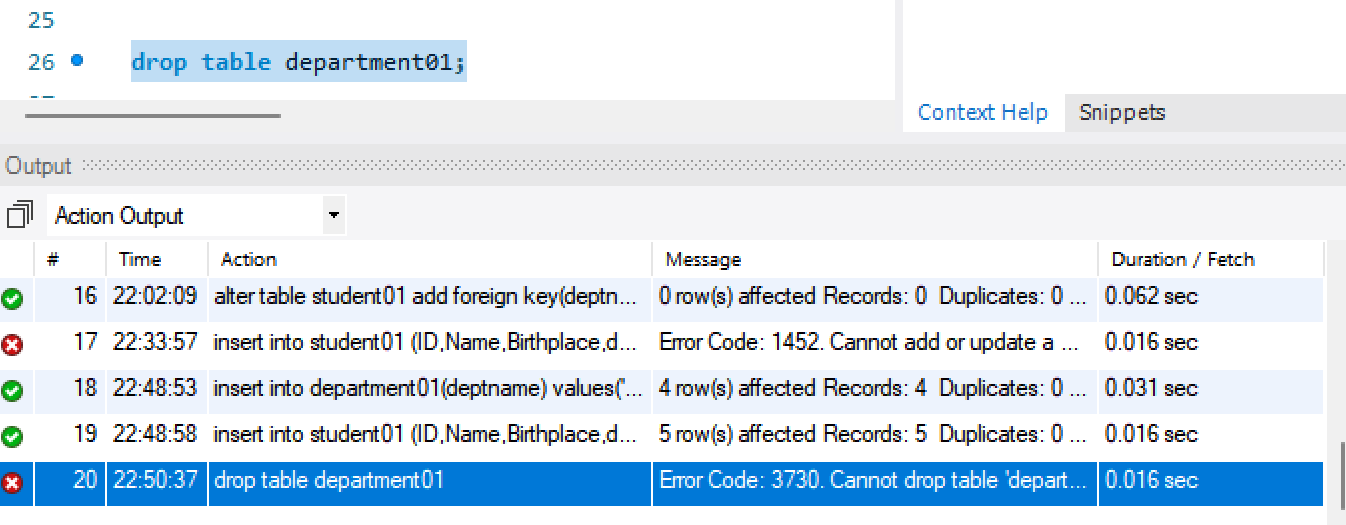
\includegraphics[width=12cm]{figure/image11.png} \\
    \footnotesize 图11 数据完整性验证操作截图
\end{center}
\vspace{1cm}

\chapter{实验总结}
\section{技术收获}
1. 掌握Python与MySQL的异常处理机制
2. 深入理解外键约束对数据完整性的保障作用
3. 熟练运用DDL和DML语句进行数据库操作
4. 学会通过错误信息定位和解决数据库操作问题

\section{典型问题处理}
\begin{enumerate}
\item \textbf{外键冲突问题}：插入数据时外键不存在导致错误，通过先插入主表数据解决。
\item \textbf{表依赖问题}：删除表时存在外键依赖，通过先删除外键约束解决。
\item \textbf{字段拼写错误}：更新语句中字段名拼写错误导致异常，通过仔细检查 SQL 语句修正。
\end{enumerate}

\section{实验启示}
通过本次实验深刻体会到：
- 数据库设计中数据完整性约束的重要性
- 开发过程中异常处理的必要性
- 数据库操作需严格遵循事务处理原则
- 版本控制工具在代码管理中的重要性

\end{spacing}
\end{document}    